\newpage
\section{Durchführung}
\label{sec:Durchführung}

\subsection{Aufbau des \ce{Ge}-Detektors}
\label{sec:AufbauDetektor}

Der verwendete Detektor ist ein sogenannter koaxialer \ce{Ge}-Detektor.
Er besteht aus einem zylinderförmigen \ce{Ge}-Kristall mit einer Bohrung in
Inneren, auf welche ein Kontakt aufgedampft ist. Von außen sind \ce{Li}-Atome
eindiffundiert, sodass die äußere Schicht von \SI{0.5}{\milli\meter} Dicke
stark n-dotiert ist.
Zwischen den Goldkontakt und die äußere dotierte Schicht lässt sich eine äußere
Spannung $U$ anlegen.
Zur Abschirmung des Detektors ist dieser Aufbau von einer Aluminium-Schutzhaub
umgeben. Als Konsequenz existiert eine untere Nachweisgrenze für $\gamma$-Quanten
von \SIrange{40}{50}{\kilo\electronvolt}.
Dieser Aufbau ist in Abbildung \ref{fig:Versuchsaufbau} dargestellt.
Hierbei strahlt die Quelle von oben auf den Detektor.
Der gesamte Aufbau befindet sich in einer Bleiverkleidung, um die Detektion
von Hintergrundstrahlung zu verhindern. Innerhalb befindet sich weiterhin eine
Platte aus hochreinem Kupfer, welche die natürliche Strahlung des Bleis vor dem
Detektor abschirmt.
\begin{figure}
	\centering
	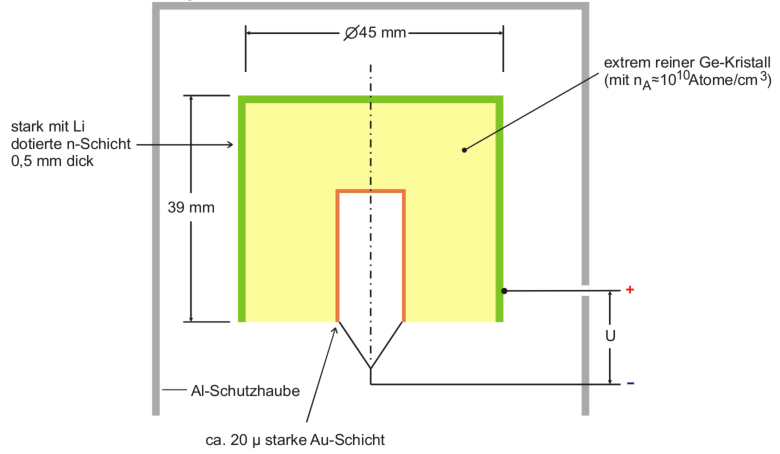
\includegraphics[width=.8\textwidth]{images/Versuchsaufbau.pdf}
	\caption{Schematische Darstellung eines koaxialen Reinst-\ce{Ge}-Detektors~\cite[14]{anleitung}.}
	\label{fig:Versuchsaufbau}
\end{figure}

Um von dem aufgenommenen Spektrum auf die Aktivität nach Formel \eqref{eqn:Vollenergie-Nachweiseffizienz}
schließen zu können, wird der Raumwinkel benötigt.
Da der Abstand $a$ zwischen Quelle und Detektor groß gegenüber der Quellenabmessung
ist, gilt der Zusammenhang
\begin{equation}
	\frac{\Omega}{2\:\pi} = \frac{1}{2} \left(1 - \frac{a}{\sqrt{a^2 + r^2}}\right)
	\label{eqn:Raumwinkel}
\end{equation}
mit dem Radius $r$ nach Abbildung \ref{fig:Raumwinkel}.
\begin{figure}
	\centering
	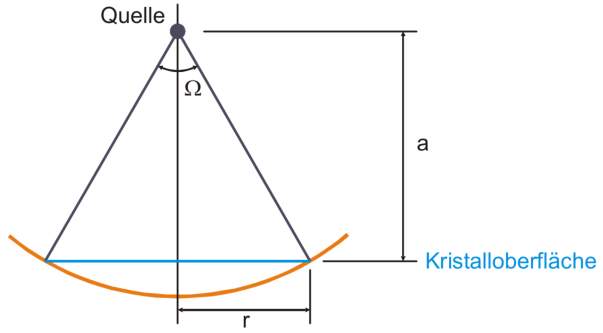
\includegraphics[width=.5\textwidth]{images/Raumwinkel.pdf}
	\caption{Skizze zur Berechnung des Raumwinkels $\Omega$~\cite[25]{anleitung}.}
	\label{fig:Raumwinkel}
\end{figure}

\subsection{Schaltung des Detektors}
\label{sec:Schaltungen}

% TODO

\subsection{Kalibrierung des Detektors}
\label{sec:KalibrierungBeschreibung}

Zuerst wird der Verstärker eingeschaltet und geprüft, ob der Detektor gekühlt ist.
Im Anschluss wird langsam die eine äußere Spannung von \SI{5}{\kilo\volt} angelegt
und der Abstandshalter mit einer Schieblehre vermessen,
welcher den Abstand zwischen Probe und Detektor festlegt.
Im Anschluss wird das Spektrum eines kalibrierten \ce{^125Eu}-Strahlers für eine Stunde aufgenommen.
Hieraus lässt sich die Energieeichung und Vollenergie-Nachweiseffizienz
des Detektors bestimmen.
Die theoretischen Emissionswahrscheinlichkeiten sind dazu in \cite[28]{anleitung} angegeben.
Die Aufnahme des Spektrums erfolgt mit Hilfe des Computerprogramms
\texttt{MAESTRO} und die erhaltenen Spektren werden als ASCII-Dateien gespeichert.

Im Anschluss wird die Europium-Probe entfernt und ein \ce{^137Cs}-Strahler eingesetzt,
um weitere Detektoreigenschaften wie die Absorptionswahrscheinlichkeit für
\ce{^137Cs}-Quanten zu bestimmen.
Hier beträgt die Messzeit ebenfalls eine Stunde.

\subsection{Charakterisierung unbekannter Proben}
\label{sec:CharakterisierungBeschreibung}

Die dritte Probe ist entweder eine \ce{^125Sb}- oder eine \ce{^133}-Quelle.
Das Spektrum wird wie auch bei der vierten Probe für eine Stunde aufgenommen
und daraus im Anschluss das vorliegende Material bestimmt.
Hierzu werden Tabellen mit verschiedenen $\gamma$-Linien und den zugehörigen
Emissionswahrscheinlichkeiten für Barium und Antimon aus \cite[28]{anleitung}
verwendet.
Die vierte Quelle ist ein unbekannter Strahler, dessen Zusammensetzung
aus dem Spektrum ermittelt werden soll.
